% !Mode:: "TeX:UTF-8"
\chapter{图片的插入方法}
\section{研究生毕业论文的插图规范}
图应有自明性。插图应与文字紧密配合,文图相符,内容正确。选图要力求精练,插图、照片应完整清晰。图中文字和数字等字号用宋体五号字。

机械工程图:采用第一角投影法,严格按照GB4457---GB131-83《机械制图》标准规定。

数据流程图、程序流程图、系统流程图等按GB1526-89标准规定。

电气图:图形符号、文字符号等应符合有关标准的规定。

流程图:必须采用结构化程序并正确运用流程框图。

对无规定符号的图形应采用该行业的常用画法。

坐标图的坐标线均用细实线,粗细不得超过图中曲线,有数字标注的坐标图,必须注明坐标单位。

照片图要求主题和主要显示部分的轮廓鲜明,便于制版。如用放大或缩小的复制品,必须清晰,反差适中。照片上应有表示目的物尺寸的标度。

引用文献图表必须标注出处。

\subsection{图题及图中说明}
每个图均应有图题(由图序和图名组成),图名在图序之后空两格排写。图序按章编排,如第1章第一个插图的图号为“图1-1”等。
图题置于图下,要求中文用宋体五号字,位置居中。有图注或其它说明时应置于图题之上。引用图应注明出处,在图题右上角加引用文献号。
图中若有分图时,分图题置于分图之下或图题之下,分图号用a)、b)等表示。

图中各部分说明应采用中文(引用的外文图除外)或数字项号,各项文字说明置于图题之上(有分图题者,置于分图题之上)。

\subsection{插图编排}
插图之前,文中必须有关于本插图的提示,如“见图1-1”、“如图1-1所示”等。插图与其图题为一个整体,不得拆开排写于两页。
插图处的该页空白不够排写该图整体时,则可将其后文字部分提前排写,将图移到次页。

\section{\LaTeX~中推荐使用的图片格式}
在\LaTeX~中应用最多的图片格式是EPS(Encapsulated PostScript)格式,它是一种专用的打印机描述语言,常用于印刷或打印输出。
EPS格式图片可通过多种方式生成,这里介绍一款功能强大的免费图片处理软件———\href{http://www.imagemagick.org/}{ImageMagick},
此软件可将其它格式图片转换为EPS格式图片,同时还可以锐化图片,使图片的局部清晰一些。

此软件对图片的格式转换操作都是在命令提示符(cmd.exe)中实现的,可以通过“开始$\to$运行$\to$输入cmd$\to$回车”或
“开始$\to$程序$\to$附件$\to$命令提示符”找到它。在命令提示符下,首先采用“盘符命令”或“cd命令”将当前目录改为待处理图片所在的目录,
在此目录下就可通过convert命令将图片转换为EPS格式,其命令的语法格式为

\indent\verb|convert [可选参数] 原文件名.原扩展名 新文件名.eps|.

若convert命令中无可选参数,则将原来的图片格式直接转换为EPS格式,对图片不进行任何处理,这也是最常用的方法。
也可以选用可选参数,可选参数有很多选择,但最常用的有如下两个:

\verb|-sharpen radius{xsigma}|———此参数用来锐化图片,一般用在图片像素不高,需要提高图片清晰度的情况下。其中radius只能为整数,
它用来确定转换命令采取哪一种锐化算法,我们可以只取radius为0;sigma为所采取算法的锐化度,它的取值为$0.1 - 3$之间的任意一个浮点数,
数值越大,锐化程度也越大,通常取为$0.1 - 3$之间;x在参数中为分隔符。
\verb|-resize geometry|———此参数用来改变图片的大小,若图片的存储空间过大,可通过此命令缩小图片尺寸,但同时也将导致图片像素降低,
其具体用法请参见\href{http://www.imagemagick.org/script/command-line-options.php#resize}{-resize geometry的官方说明}。

除此之外,一些文字处理软件和科学计算软件也支持生成EPS格式的文件,请使用“另存为”功能查看某款软件是否能够将图片以EPS格式的形式保存。

\section{单张图片的插入方法}
单张图片独自占一行的插入形式如图\ref{fig:xml}所示。
\begin{figure}[htbp]
	\centering
	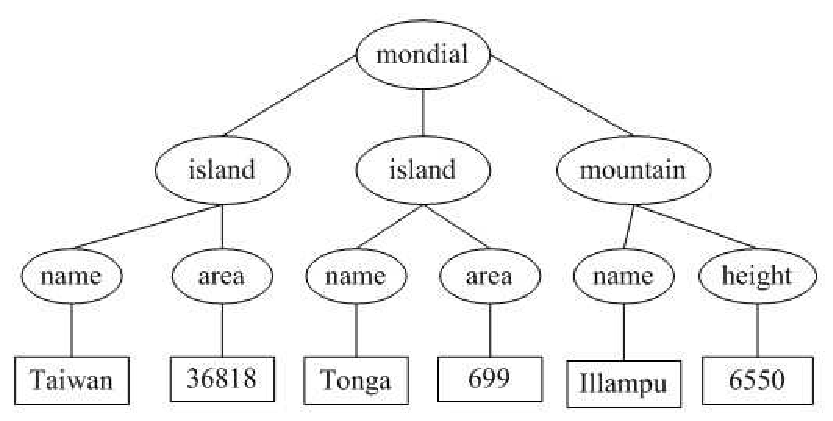
\includegraphics[width=0.4\textwidth]{XML}
	\caption{树状结构}\label{fig:xml}
	\vspace{\baselineskip}
\end{figure}


其插入图片的代码及其说明如下。
\vspace{1em}\noindent\hrule
\begin{verbatim}
	\begin{figure}[htbp]
		\centering
		\includegraphics[width=0.4\textwidth]{文件名(.eps)}
		\caption{标题}\label{标签名(通常为 fig:labelname)}
		\vspace{\baselineskip} %表示图与正文空一行
	\end{figure}
\end{verbatim}

\noindent\hrule

\begin{verbatim}
figure环境的可选参数[htbp]表示浮动图形所放置的位置,h (here)
表示当前位置,t (top)表示页芯顶部,b (bottom)表示页芯底部,
p (page)表示单独一页。在Word等软件中,图片通常插入到当前位置,
如果当前页的剩余空间不够,图片将被移动到下一页,当前页就会出现
很大的空白,其人工调整工作非常不便。由LaTeX提供的浮动图片功能,
总是会按h->t->b->p的次序处理选项中的字母,自动调整图片的位置,
大大减轻了工作量。\centering命令将后续内容转换成每行皆居中的格式。
"\includegraphics"的可选参数用来设置图片插入文中的水平宽度,
一般表示为正文宽度(\textwidth)的倍数。	\caption命令可选
参数“标签名”为英文形式,一般不以图片或表格的数字顺序作为标签,
而应包含一定的图片或表格信息,以便于文中引用(若图片、表格、公
式、章节和参考文献等在文中出现的先后顺序发生了变化,其标注序号
及其文中引用序号也会跟着发生变化,这一点是Word等软件所不能做到
的)。另外,图题或表题并不会因为分页而与图片或表格体分置于两页,
章节等各级标题也不会置于某页的最底部,LaTeX系统会自动调整它们在
正文中的位置,这也是Word等软件所无法匹敌的。\vspace将产生一定
高度的竖直空白,必选参数为负值表示将后续文字位置向上提升,参数
值可自行调整。em为长度单位,相当于大写字母M的宽度。
\vspace{\baselineskip} 表示图与正文空一行。
引用方法:“见图\ref{fig:figname}”、“如图\ref{fig:figname}所示”等。
\end{verbatim}

\noindent\hrule\vspace{1em}

若需要将2张及以上的图片并排插入到一行中,则需要采用\verb|minipage|环境,如图\ref{fig:dd}和图\ref{fig:ds}所示。
\begin{figure}[htbp]
	\centering
	\begin{minipage}{0.4\textwidth}
		\centering
		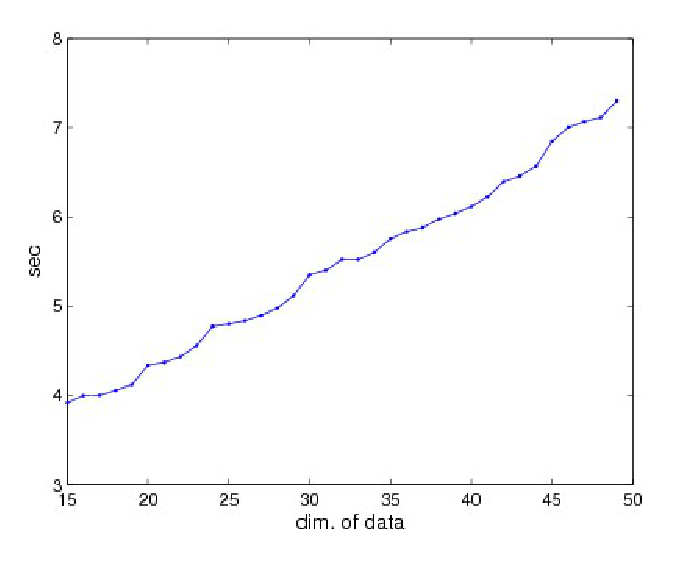
\includegraphics[width=\textwidth]{dataDimensions}
		\caption{数据维数的变化}\label{fig:dd}
	\end{minipage}
	\begin{minipage}{0.4\textwidth}
		\centering
		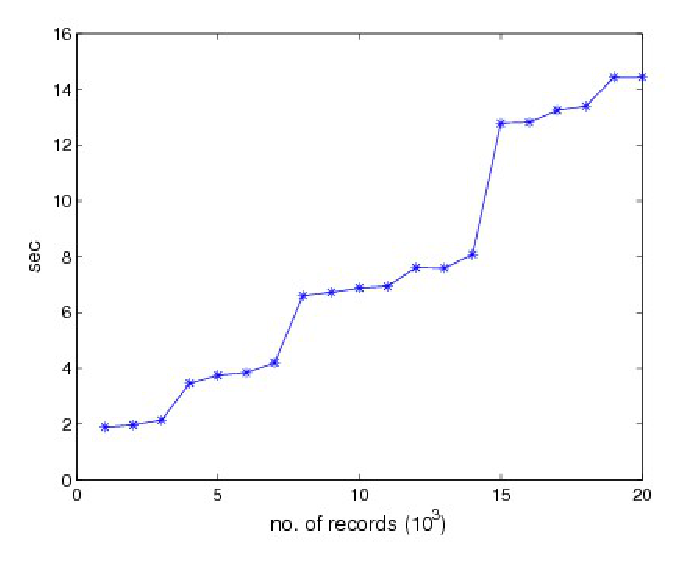
\includegraphics[width=\textwidth]{dataSize}
		\caption{数据规模的变化}\label{fig:ds}
	\end{minipage}
	\vspace{\baselineskip}
\end{figure}

其代码如下所示。

\vspace{1em}\noindent\hrule
\begin{verbatim}
	\begin{figure}[htbp]
		\centering
		\begin{minipage}{0.4\textwidth}
			\centering
			\includegraphics[width=\textwidth]{文件名}
			\caption{标题}\label{fig:f1}
		\end{minipage}
		\begin{minipage}{0.4\textwidth}
			\centering
			\includegraphics[width=\textwidth]{文件名}
			\caption{标题}\label{fig:f2}
		\end{minipage}\vspace{\baselineskip}
	\end{figure}
\end{verbatim}

\noindent\hrule

\begin{verbatim}
minipage环境的必选参数用来设置小页的宽度,若需要在一行中插入
n个等宽图片,则每个小页的宽度应略小于(1/n)\textwidth。
\end{verbatim}

\noindent\hrule

\section{具有子图的图片插入方法}
图中若含有子图时,需要调用subfigure宏包, 如图\ref{fig:subfig}所示。
\begin{figure}[htbp]
	\centering
	\subfigure[Data Dimensions]{\label{fig:subfig:datadim}
		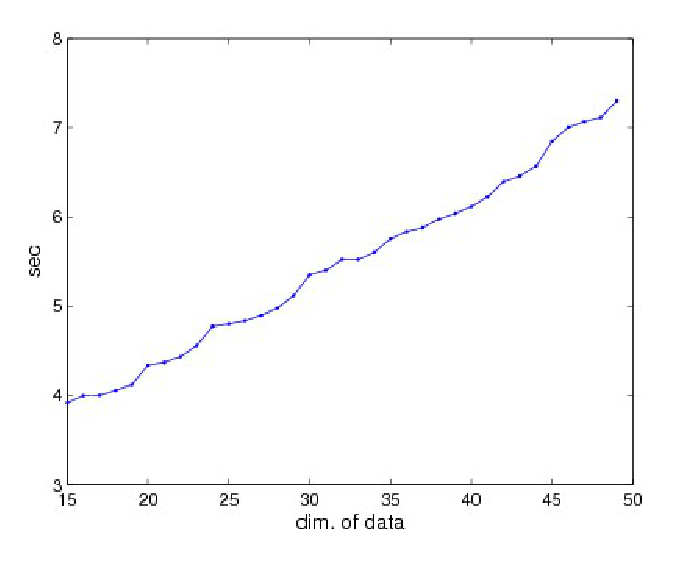
\includegraphics[width=0.4\textwidth]{dataDimensions}}
	\subfigure[Data Size]{\label{fig:subfig:datasize}
		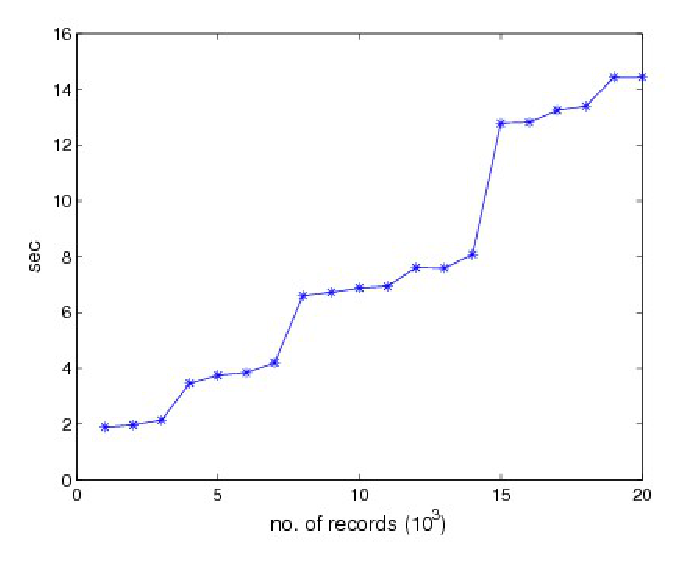
\includegraphics[width=0.4\textwidth]{dataSize}}
	\caption{Scalability of data}\label{fig:subfig}
	\vspace{\baselineskip}
\end{figure}

其代码及其说明如下。
\vspace{1em}\noindent\hrule

\begin{verbatim}
	\begin{figure}[htbp]
		\centering
		\subfigure[第1个子图标题]{
			\label{第1个子图标签(通常为 fig:subfig1:subsubfig1)}
			\includegraphics[width=0.4\textwidth]{文件名}}
		\subfigure[第2个子图标题]{
			\label{第2个子图标签(通常为 fig:subfig1:subsubfig2)}
			\includegraphics[width=0.4\textwidth]{文件名}}
		\caption{总标题}\label{总标签(通常为 fig:subfig1)}
		\vspace{\baselineskip}
	\end{figure}
\end{verbatim}

\noindent\hrule

\begin{verbatim}
	子图的标签实际上可以随意设定,只要不重复就行。但为了更好的
	可读性,我们建议fig:subfig:subsubfig格式命名,这样我们
	从标签名就可以知道这是一个子图引用。引用方法:总图的引用方
	法同本章第1节,子图的引用方法用\ref{fig:subfig:subsubfig}
	来代替。
\end{verbatim}

\noindent\hrule\vspace{1em}

子图的引用示例:如图\ref{fig:subfig:datadim}和图\ref{fig:subfig:datasize}所示。

若想获得插图方法的更多信息,参见网络上的\href{ftp://ftp.tex.ac.uk/tex-archive/info/epslatex.pdf}{Using Imported Graphics in \LaTeX~ and pdf\LaTeX~}文档。